\documentclass{article}

%%%%%%%%%%%%%%%%%%%%%%%%%%%%%%%%%%%%%%%%%%%%%%%%%%%%%%%%%%%%%%%%%%%%%%%

\usepackage{url}
\usepackage{graphicx}

% Remove red border around refs and make them stand out.
\usepackage[colorlinks=true,linkcolor=blue]{hyperref}

%%%%%%%%%%%%%%%%%%%%%%%%%%%%%%%%%%%%%%%%%%%%%%%%%%%%%%%%%%%%%%%%%%%%%%%
%% Check these macro values for appropriateness for your own document.

\title{IS3 Group Report}

%%authors
\author{
  Richard Fleming \\
  James Gallagher \\
  Craig McLaughlin \\
  Victor Pantazi \\
  Gordon Reid \\
  Ross Taylor}

%%release date 
\date{\today}

%%%%%%%%%%%%%%%%%%%%%%%%%%%%%%%%%%%%%%%%%%%%%%%%%%%%%%%%%%%%%%%%%%%%%%%

\begin{document}

%%%%%%%%%%%%%%%%%%%%%%%%%%%%%%%%%%%%%%%%%%%%%%%%%%%%%%%%%%%%%%%%%%%%%%%

\maketitle

%%%%%%%%%%%%%%%%%%%%%%%%%%%%%%%%%%%%%%%%%%%%%%%%%%%%%%%%%%%%%%%%%%%%%%%
%% Standard section for all documents

\section{Preamble}

In this report, various popular calendars are evaluated using the
Think-aloud evaluation technique to identify desirable features of a
modern calendar. Three paper prototypes are designed by pairs from the
team, and based on these paper prototypes, a final paper prototype will
be detailed.


\begin{itemize}
\item Give an overview of your paper prototypes, the early designs and
how you came to your final prototype design;

\item Explain how they work;

\item Report on your heuristic evaluation/think aloud, any problems you
found and how you resolved them (include the key paper prototypes that
you built);
\end{itemize}

\section{Overview}

Our prototypes were based on the Facebook, OS X, Evolution on Scientific
Linux, and Google calendars. For prototyping and evaluating we split up
into two person teams. For the purposes of the discussion the teams are
labelled based on the calendars they evaluated.

The final paper prototype was a combination of our findings from the
calendars.

\section{Calendar on OS X}

Apple Inc.'s use of skeuomorphism creates an interface similar to a real 
calendar with simulated page rips, faux-leather textures for UI
elements, and page turn animations. The design of the paper prototype
based on this calendar borrowed from the ethos of Apple's design.

\subsection{Think-aloud Evaluation}
The participant was asked to perform a series of set tasks, incorporated
into a scenario. Below the tasks are described and feedback from the
participant noted:

\begin{itemize}
\item Add an event for a friends party.

There was an intuitive plus button on the top-left of the window, which
opened a dialog box for adding an event on the currently selected day.

\item Change the event to the following week.

\item Delete the event.

\item Set a recurring event.

\item Find out which days of the month are the busiest and quietest
respectively

The year view for the calendar fills days in colour indicating the
number of appointments scheduled for that day, in a spectrum from
red (busy) to white (quiet). This made this particular task incredibly
simple and it is this reason this feature was included in an early
paper prototype (see Section~\ref{sec:osxpp}).

\item Change the calendar catergories currently displayed.
\end{itemize}

The participant noted feeling uncomfortable during the evaluation as it
was unnatural for the them to have to vocalise their actions. At some
points during the experiment, the participant seemed confused or
surprised by the feedback from the system, occasionally expressing
uncertainty on how to proceed further with the task.

\subsection{Paper prototypes}
\label{sec:osxpp}

The paper prototype has a minimalist design with three views: week,
month, and year. These views are available through three buttons that
are always on the screen at the top centre-right. The currently selected
view is coloured differently than the others and appears depressed.

The initial draft of the event dialog pop up window, that would be
shown when a user decides to add a new event, or wishes to edit or
delete an existing event, is illustrated in Figure~\ref{fig:addevent}.

A user is able to have multiple calendars, perhaps to split up work and
home events. This screen (Figure~\ref{fig:viewcal}) allows a user to
choose which calendars to view, add a new calendar, or delete an old
calendar and associated events.

The month view for our calendar is shown in Figure~\ref{fig:monthview}.
This view is also the default view. Events are listed in summary form
in the grid of squares. When a user clicks on the grid, the full listing
for the selected day is shown in the side panel on the right.

The year view for our calendar is depicted in Figure~\ref{fig:yearview}.
The primary purpose of the view is to allow daily summaries to be
visualised. Similar to Apple's Calendar application, days which are
busy are coloured in an increasing level of opaqueness, dependant on
the number of events added for the associated day.

\section{Evolution on Scientific Linux}

This paper prototype was designed using our findings from our evaluation 
of Evolution on Scientific Linux.

The first thing we noticed about Evolution was that there wasn't always
a clear indication of the current system state so for our prototype we
included a clear `Day/Week/Month/Year' section at the top of the screen
which also allowed the user to quickly switch between views. Another
indicator of system state we added was a check box section on the left of
the main view to allow users to select different categories of event to
be displayed. Also related to event categories, we found Evolution's
system for adding a new category to be rather unintuitive so we added a
clear indication in the categories section of the sidebar labelled
'Add New'. We also didn't like the inconsistencies we found whilst
using the Evolution system so we decided the different views in our
prototype should have the same features available (i.e the sidebar
feature and the view indicator).

\subsection{Problems during Evaluation}


%%%%%%%%%

See figures (need figures).
\section{The Video}

\url{http://www.youtube.com/watch?v=yAREKMqu538}

%% Separate sections with line of comment symbols.
%%%%%%%%%%%%%%%%%%%%%%%%%%%%%%%%%%%%%%%%%%%%%%%%%%%%%%%%%%%%%%%%%%%%%%%

\appendix
\section{Figures for Calendar on OS X}

\begin{figure}
\centering
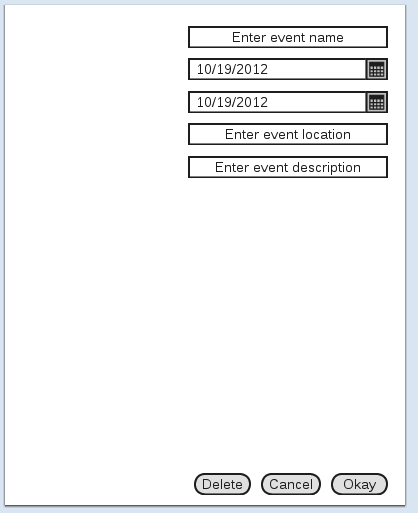
\includegraphics[height=9cm,width=9.5cm]{CMCLGDREvent.png}
\caption{Add Event dialog}
\label{fig:addevent}
\end{figure}

\begin{figure}
\centering
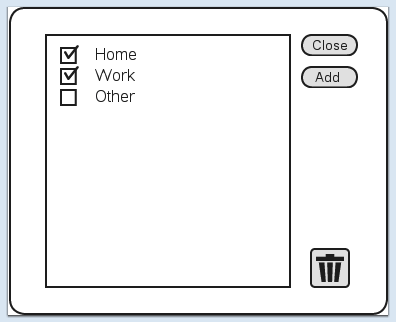
\includegraphics[height=8cm,width=8.5cm]{CMCLGDRViewCalendar.png}
\caption{View Calendar Dialog}
\label{fig:viewcal}
\end{figure}

\begin{figure}
\centering
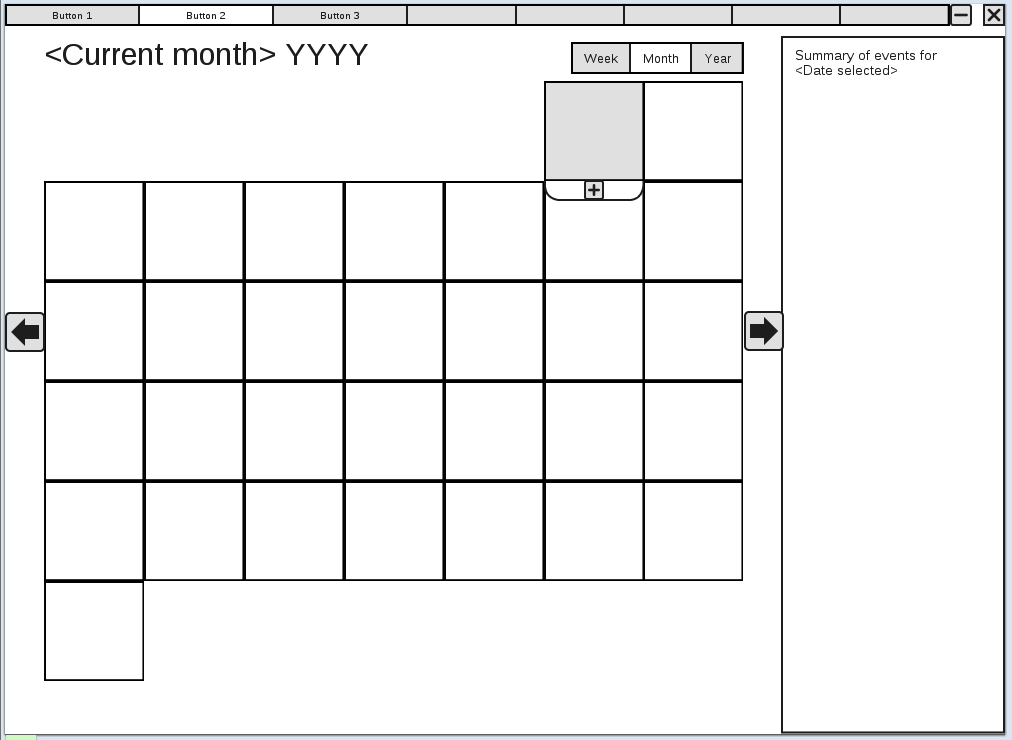
\includegraphics[scale=0.5,angle=90]{CMCLGDRMonth.png}
\caption{Month View}
\label{fig:monthview}
\end{figure}

\begin{figure}
\centering
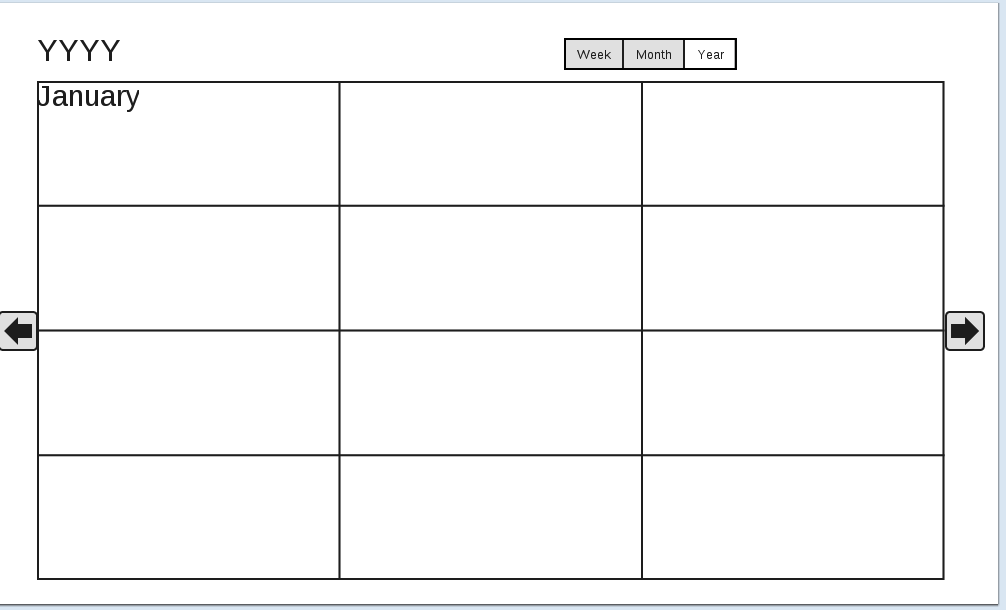
\includegraphics[scale=0.5,angle=90]{CMCLGDRYear.png}
\caption{Year View}
\label{fig:yearrview}
\end{figure}

\end{document}

%%%%%%%%%%%%%%%%%%%%%%%%%%%%%%%%%%%%%%%%%%%%%%%%%%%%%%%%%%%%%%%%%%%%%%%
